\documentclass{article}

%%%%%%%%%%%%%%%%%%%%%%%%%%%%%%%%%%%%%%%%%
% Lachaise Assignment
% Structure Specification File
% Version 1.0 (26/6/2018)
%
% This template originates from:
% http://www.LaTeXTemplates.com
%
% Authors:
% Marion Lachaise & François Févotte
% Vel (vel@LaTeXTemplates.com)
%
% License:
% CC BY-NC-SA 3.0 (http://creativecommons.org/licenses/by-nc-sa/3.0/)
% 
%%%%%%%%%%%%%%%%%%%%%%%%%%%%%%%%%%%%%%%%%

%----------------------------------------------------------------------------------------
%	PACKAGES AND OTHER DOCUMENT CONFIGURATIONS
%----------------------------------------------------------------------------------------

\usepackage{amsmath,amsfonts,stmaryrd,amssymb} % Math packages

\usepackage{enumerate} % Custom item numbers for enumerations

\usepackage[ruled]{algorithm2e} % Algorithms

\usepackage[framemethod=tikz]{mdframed} % Allows defining custom boxed/framed environments

\usepackage{listings} % File listings, with syntax highlighting
\lstset{
	basicstyle=\ttfamily, % Typeset listings in monospace font
}

%----------------------------------------------------------------------------------------
%	DOCUMENT MARGINS
%----------------------------------------------------------------------------------------

\usepackage{geometry} % Required for adjusting page dimensions and margins

\geometry{
	paper=a4paper, % Paper size, change to letterpaper for US letter size
	top=2.5cm, % Top margin
	bottom=3cm, % Bottom margin
	left=2.5cm, % Left margin
	right=2.5cm, % Right margin
	headheight=14pt, % Header height
	footskip=1.5cm, % Space from the bottom margin to the baseline of the footer
	headsep=1.2cm, % Space from the top margin to the baseline of the header
	%showframe, % Uncomment to show how the type block is set on the page
}

%----------------------------------------------------------------------------------------
%	FONTS
%----------------------------------------------------------------------------------------

\usepackage[utf8]{inputenc} % Required for inputting international characters
\usepackage[T1]{fontenc} % Output font encoding for international characters

\usepackage{XCharter} % Use the XCharter fonts

%----------------------------------------------------------------------------------------
%	COMMAND LINE ENVIRONMENT
%----------------------------------------------------------------------------------------

% Usage:
% \begin{commandline}
%	\begin{verbatim}
%		$ ls
%		
%		Applications	Desktop	...
%	\end{verbatim}
% \end{commandline}

\mdfdefinestyle{commandline}{
	leftmargin=10pt,
	rightmargin=10pt,
	innerleftmargin=15pt,
	middlelinecolor=black!50!white,
	middlelinewidth=2pt,
	frametitlerule=false,
	backgroundcolor=black!5!white,
	frametitle={Command Line},
	frametitlefont={\normalfont\sffamily\color{white}\hspace{-1em}},
	frametitlebackgroundcolor=black!50!white,
	nobreak,
}

% Define a custom environment for command-line snapshots
\newenvironment{commandline}{
	\medskip
	\begin{mdframed}[style=commandline]
}{
	\end{mdframed}
	\medskip
}

%----------------------------------------------------------------------------------------
%	FILE CONTENTS ENVIRONMENT
%----------------------------------------------------------------------------------------

% Usage:
% \begin{file}[optional filename, defaults to "File"]
%	File contents, for example, with a listings environment
% \end{file}

\mdfdefinestyle{file}{
	innertopmargin=1.6\baselineskip,
	innerbottommargin=0.8\baselineskip,
	topline=false, bottomline=false,
	leftline=false, rightline=false,
	leftmargin=2cm,
	rightmargin=2cm,
	singleextra={%
		\draw[fill=black!10!white](P)++(0,-1.2em)rectangle(P-|O);
		\node[anchor=north west]
		at(P-|O){\ttfamily\mdfilename};
		%
		\def\l{3em}
		\draw(O-|P)++(-\l,0)--++(\l,\l)--(P)--(P-|O)--(O)--cycle;
		\draw(O-|P)++(-\l,0)--++(0,\l)--++(\l,0);
	},
	nobreak,
}

% Define a custom environment for file contents
\newenvironment{file}[1][File]{ % Set the default filename to "File"
	\medskip
	\newcommand{\mdfilename}{#1}
	\begin{mdframed}[style=file]
}{
	\end{mdframed}
	\medskip
}

%----------------------------------------------------------------------------------------
%	NUMBERED QUESTIONS ENVIRONMENT
%----------------------------------------------------------------------------------------

% Usage:
% \begin{question}[optional title]
%	Question contents
% \end{question}

\mdfdefinestyle{question}{
	innertopmargin=1.2\baselineskip,
	innerbottommargin=0.8\baselineskip,
	roundcorner=5pt,
	nobreak,
	singleextra={%
		\draw(P-|O)node[xshift=1em,anchor=west,fill=white,draw,rounded corners=5pt]{%
		Question \theQuestion\questionTitle};
	},
}

\newcounter{Question} % Stores the current question number that gets iterated with each new question

% Define a custom environment for numbered questions
\newenvironment{question}[1][\unskip]{
	\bigskip
	\stepcounter{Question}
	\newcommand{\questionTitle}{~#1}
	\begin{mdframed}[style=question]
}{
	\end{mdframed}
	\medskip
}

%----------------------------------------------------------------------------------------
%	WARNING TEXT ENVIRONMENT
%----------------------------------------------------------------------------------------

% Usage:
% \begin{warn}[optional title, defaults to "Warning:"]
%	Contents
% \end{warn}

\mdfdefinestyle{warning}{
	topline=false, bottomline=false,
	leftline=false, rightline=false,
	nobreak,
	singleextra={%
		\draw(P-|O)++(-0.5em,0)node(tmp1){};
		\draw(P-|O)++(0.5em,0)node(tmp2){};
		\fill[black,rotate around={45:(P-|O)}](tmp1)rectangle(tmp2);
		\node at(P-|O){\color{white}\scriptsize\bf !};
		\draw[very thick](P-|O)++(0,-1em)--(O);%--(O-|P);
	}
}

% Define a custom environment for warning text
\newenvironment{warn}[1][Warning:]{ % Set the default warning to "Warning:"
	\medskip
	\begin{mdframed}[style=warning]
		\noindent{\textbf{#1}}
}{
	\end{mdframed}
}

%----------------------------------------------------------------------------------------
%	INFORMATION ENVIRONMENT
%----------------------------------------------------------------------------------------

% Usage:
% \begin{info}[optional title, defaults to "Info:"]
% 	contents
% 	\end{info}

\mdfdefinestyle{info}{%
	topline=false, bottomline=false,
	leftline=false, rightline=false,
	nobreak,
	singleextra={%
		\fill[black](P-|O)circle[radius=0.4em];
		\node at(P-|O){\color{white}\scriptsize\bf i};
		\draw[very thick](P-|O)++(0,-0.8em)--(O);%--(O-|P);
	}
}

% Define a custom environment for information
\newenvironment{info}[1][Info:]{ % Set the default title to "Info:"
	\medskip
	\begin{mdframed}[style=info]
		\noindent{\textbf{#1}}
}{
	\end{mdframed}
}
 % Include the file specifying the document structure and custom commands

%----------------------------------------------------------------------------------------
%	ASSIGNMENT INFORMATION
%----------------------------------------------------------------------------------------

\title{MAT2040: Project \#2} % Title of the assignment

\author{Lingxiao XU\\ \texttt{119020061}} % Author name and email address

\date{The Chinese University of HongKong, shenzhen --- \today} % University, school and/or department name(s) and a date

%----------------------------------------------------------------------------------------

\begin{document}

\maketitle 

%----------------------------------------------------------------------------------------
%	PATR 1
%----------------------------------------------------------------------------------------

\section*{PART 1} 

We need to build a model to predict the product price in this project. This project took the product price on a daily basis, which means each price was collected on consecutive days. Firstly, a data visualization of the training data was performed.
\begin{figure}[htbp]\centering
	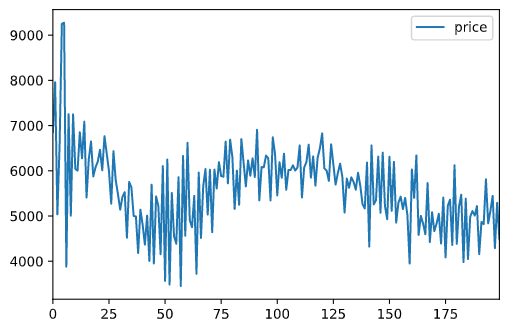
\includegraphics[width=6.5cm]{Part1_trainingData.png}
	\caption{The data visualization of the part 1 training data}
	\label{fig:part1_training}
\end{figure}

\subsection*{Model 1: Autoregressive Model}
The Autoregressive Model Specifies that the dependent variable depends on its own previous values, which means we could use its past values to predict the future values.
\\The notation AR(p) indicates an Autoregressive model of order p, which means the model uses p lags of time slots to predict the dependent variable
% Math equation/formula
\begin{equation}
	X_{t} = c + \sum_{i=1}^{p}\varphi_{t}X_{t-i} + \varepsilon_{t} \label{1}
\end{equation}

The estimation of the coefficients in this model could be done by finding the least squares estimation of the following system
\begin{equation}
\left[
\begin{array}[]{c}
	X_{p+1} \\
	X_{p+2} \\
	X_{p+3} \\
	\vdots  \\
	X_{n} 
\end{array}
\right]
=
\left[
\begin{matrix}
	1  &X_{1}  &X_{2}  &X_{3} &\cdots &X_{p} \\
	1  &X_{2}  &X_{3}  &X_{4} &\cdots &X_{p+1} \\
	1  &X_{3}  &X_{4}  &X_{5} &\cdots &X_{p+2} \\
	1  &\vdots &\vdots &\vdots&\ddots &\vdots \\
	1  &X_{n-p-1} &X_{n-p} &X_{n-p+1} &\cdots &X_{n-1} 
\end{matrix}
\right]
\left[
\begin{array}[]{c}
	c \\
	\varphi_{1} \\
	\varphi_{2} \\
	\varphi_{3} \\
	\vdots \\
	\varphi_{p}
\end{array}
\right]
\end{equation}

\begin{info} % Information block
	Other methods like The Yule Walker Equations could also be used to estimate the coefficients of autoregression model.
\end{info}

\subsubsection{Lags Selection} 
The key question in this model is to determine how many lags should be taken into the model, which is the value of p in the model. This project used two standards to select time lags, which are auto correlation function(ACF) and partial auto correlation function(PACF)\\
\\
\textbf{Auto Correlation Function (ACF)}\\
ACF describes the autocorrelation between an observation and another observation at a prior time step that includes direct and indirect dependence information.
This means we would expect the ACF for the AR(k) time series to be strong to a lag of k and the inertia of that relationship would carry on to subsequent lag values, trailing off at some point as the effect was weakened.

\begin{equation}
	R_{xx}(t_{1}, t_{2}) = E[X_{t1}\overline{X_{t2}}]
\end{equation}

\begin{figure}[htbp]\centering
	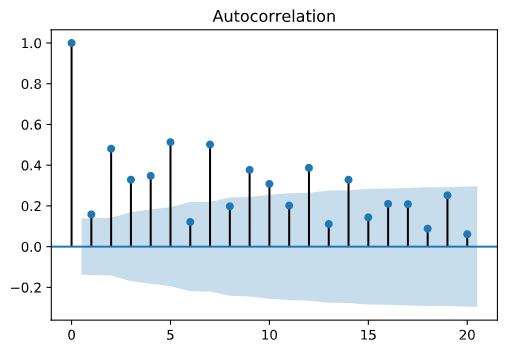
\includegraphics[width=6.5cm]{ACF.png}
	\caption{ACF of part 1 training data}
	\label{fig: ACF}
\end{figure}

The figure shows that the AR(10) time series has statistically significant relationship.
\\
\\
\textbf{Partial Auto Correlation Function (PACF)}\\
The partial autocorrelation at lag k is the correlation that results after removing the effect of any correlations due to the terms at shorter lags.\\
Given a time series $Z_{t}$, the partial autocorrelation of lag k, denoted as $\alpha_{k}$, is the autocorrelation between $Z_{t}$ and $Z_{t+k}$ with the linear dependence of $Z_{t}$ on $Z_{t+k-1}$ removed;
equivalently, it is the autocorrelation between $Z_{t}$ and $Z_{t+k}$ that is not accounted for by lag 1 through $t+k-1$, inclusive.\\
\begin{equation}
	\alpha(1) = corr(Z_{t+1}, Z_{t}), for k = 1
\end{equation}
\begin{equation}
	\alpha(k) = corr(Z_{t+k} - P_{t,k}(Z_{t+k}), Z_{t} - P_{t,k}(Z_{t})), for k \geq 2
\end{equation}
where $P_{t,k} (x)$ is the orthogonal projection of x onto the linear subspace spanned by $Z_{t+1}$, $\cdot$, $Z_{t+k+1}$.

\begin{figure}[htbp]\centering
	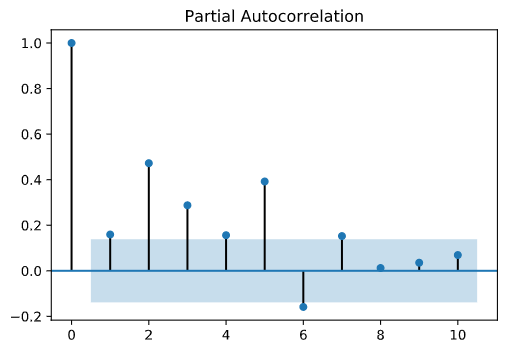
\includegraphics[width=6.5cm]{PACF.png}
	\caption{PACF of part 1 training data}
	\label{fig: PACF}
\end{figure}

By considering ACF and BACF, this report selected lag1, lag2, lag3, lag4, lag5, and lag6, which means p=6 in equation (1).

\subsubsection{Implementation and Prediction}
This project used AutoReg function from statsmodels package to implement and predict the model. The result of the regression is presented as follows:\\
\begin{figure}[htbp]\centering
	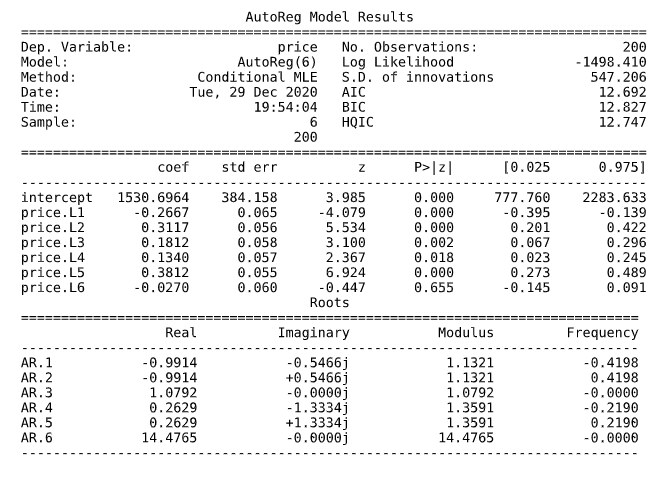
\includegraphics[width=8cm]{Auto_res.png}
	\caption{The result of the autoregression model}
	\label{fig: Auto regression}
\end{figure}
\\
Based on this model, we could predict the product price in 100 days. The result is presented as follows:
\begin{figure}[htbp]\centering
	\centering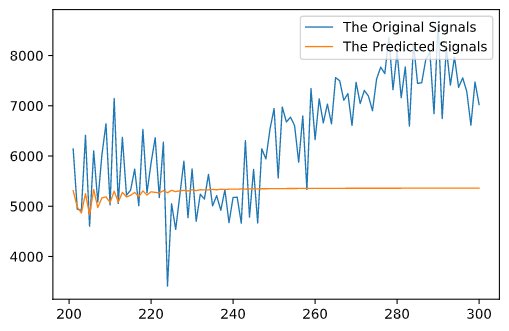
\includegraphics[width=6.5cm]{AutoReg_res1.png}
	\caption{The predicted price and the true price}
	\label{fig: AutoReg_res}
\end{figure}

\begin{figure}[htbp]\centering
	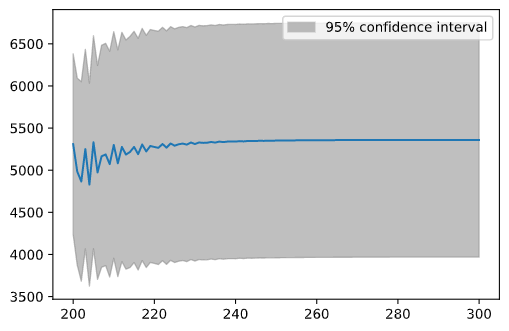
\includegraphics[width=6.5cm]{Auto_Conf.png}
	\caption{The Prediction Confidence Interval}
	\label{fig: Auto regression}
\end{figure}

The RMSE of this model is 1481.368.

\begin{equation}
	RMSE = \sqrt{\frac{1}{N}\sum_{i=1}^{N}\varepsilon_{i}^{2}}
\end{equation}

\subsubsection{Validation of the Model}
The least squares estimation of the autoregression model relies on several assumptions
\begin{itemize}
	\item [1)] \textbf{Homoscedasticity}: The variance of the residual is the same.
	\item [2)] \textbf{Independence}: The error terms are not correlated.
	\item [3)] \textbf{Normality}: For any fixed value of regressors, the dependent variable is normality distributed.
\end{itemize}
The following figure can well verify whether the model satisfies the above assumptions.\\
\begin{figure}[htbp]\centering
	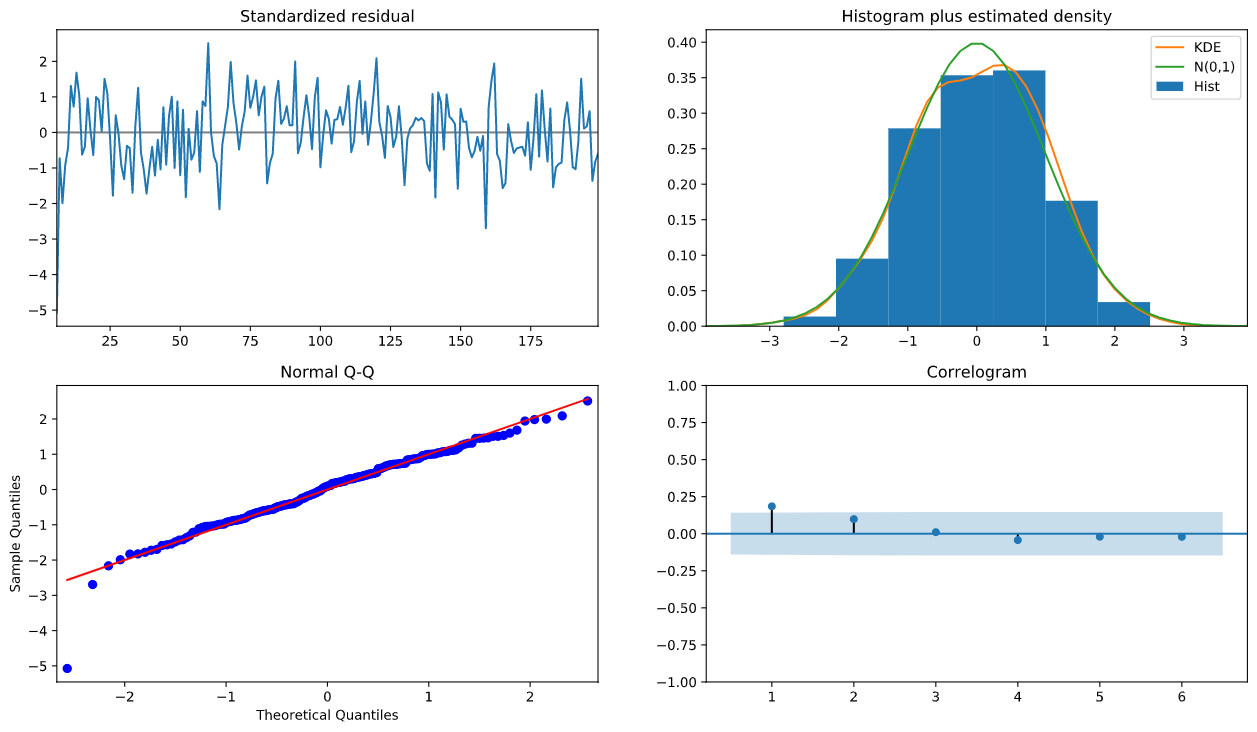
\includegraphics[width=15cm]{Autoreg_Assump.png}
	\caption{The Validation of the Assumptions}
	\label{fig: Auto regression}
\end{figure}
\\The first graph indicates that the residuals are not correlated with regressors The Second and third graph indicate that the dependent variable and regressors have finite fourth moments, and it meets the normality(residuals are normally distributed) as well as homoscedasticity assumptions in regression. The fourth graph indicates that there are no new auto correlated regressors should be taken into consideration(The chosen regressors are comprehensive enough)


\subsection*{Model 2: Fourier Series}
The Fourier transform transforms a function of time and signal into a function of frequency and power. Real data often contains noise and Fourier transform makes it easy to see through the noise. Since the price of the product is a discrete time series, this report used discrete transform. The mathematics is presented as follows:
\begin{equation}
	X_{k} = \sum_{n=0}^{N-1}x_{n}e^{-\frac{i2\pi}{N}kn} \\
		  = \sum_{n=0}^{N-1}x_{n}\left[\cos\left(\frac{2\pi}{N}kn\right)-i\sin\left(\frac{2\pi}{N}kn\right)\right]
\end{equation}
In order to perform a prediction, this project firstly run a simple linear regression of the price on time. If the price has a periodic characteristic, its residuals should tend to be periodic. This project performs a Fourier transform on the residuals and take the Fourier terms into regression to calculate the Fourier coefficients.
The R-squared of the regression model is 9.01e - 0.2.\\
Next, by performing a Fourier transformation, the dominant frequencies could be found.
\begin{figure}[htbp]\centering
	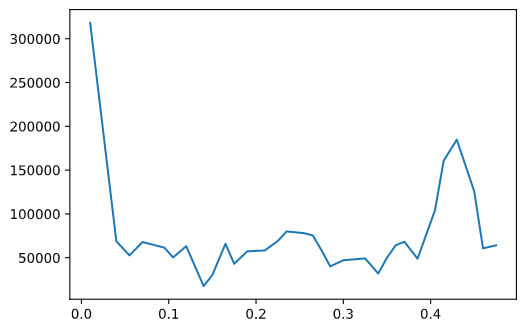
\includegraphics[width=6.5cm]{Fourier_Freq.png}
	\caption{The Dominant Frequencies}
	\label{fig: Fourier Transform}
\end{figure}
Here are the values these peaks correspond to.\\
\begin{figure}[htbp]\centering
	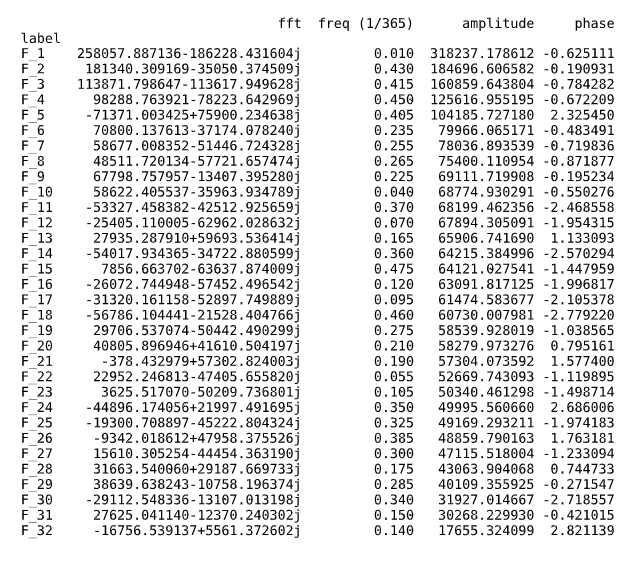
\includegraphics[width=10cm]{Fourier_terms.png}
	\caption{The fourier terms}
	\label{fig: Fourier Transform}
\end{figure}
\\
The first simple linear regression only considers the time as regressor. After performing Fourier transform, fourier terms could be added into regression.
The new term should be the function of the form:
\\
\begin{equation}
	f(t) = A\cos(\omega t + \phi )
\end{equation}
\\
A is the amplitude, $\omega$ is the angular frequency, and $\phi$ is the phase shift.\\
The fourier terms in figure 9 is the waves corresponding each peak. For example, the relationship between time and the first wave is presented as follows:
\\
\begin{figure}[htbp]\centering
	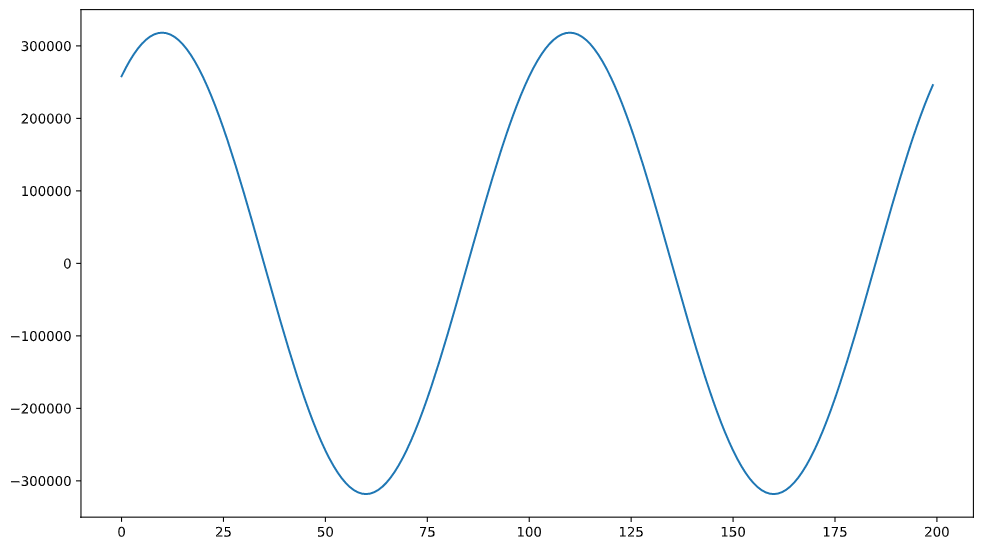
\includegraphics[width=6.5cm]{wave1.png}
	\caption{The relationship between time and $F_1$}
	\label{fig: Fourier Transfrom}	
\end{figure}
\\
Then, adding each waves from the Fourier transform into one column.
Finally, include these terms into linear regression, the predicted value on the training data and the true value looks like:
\\
\\
\begin{figure}[htbp]\centering
	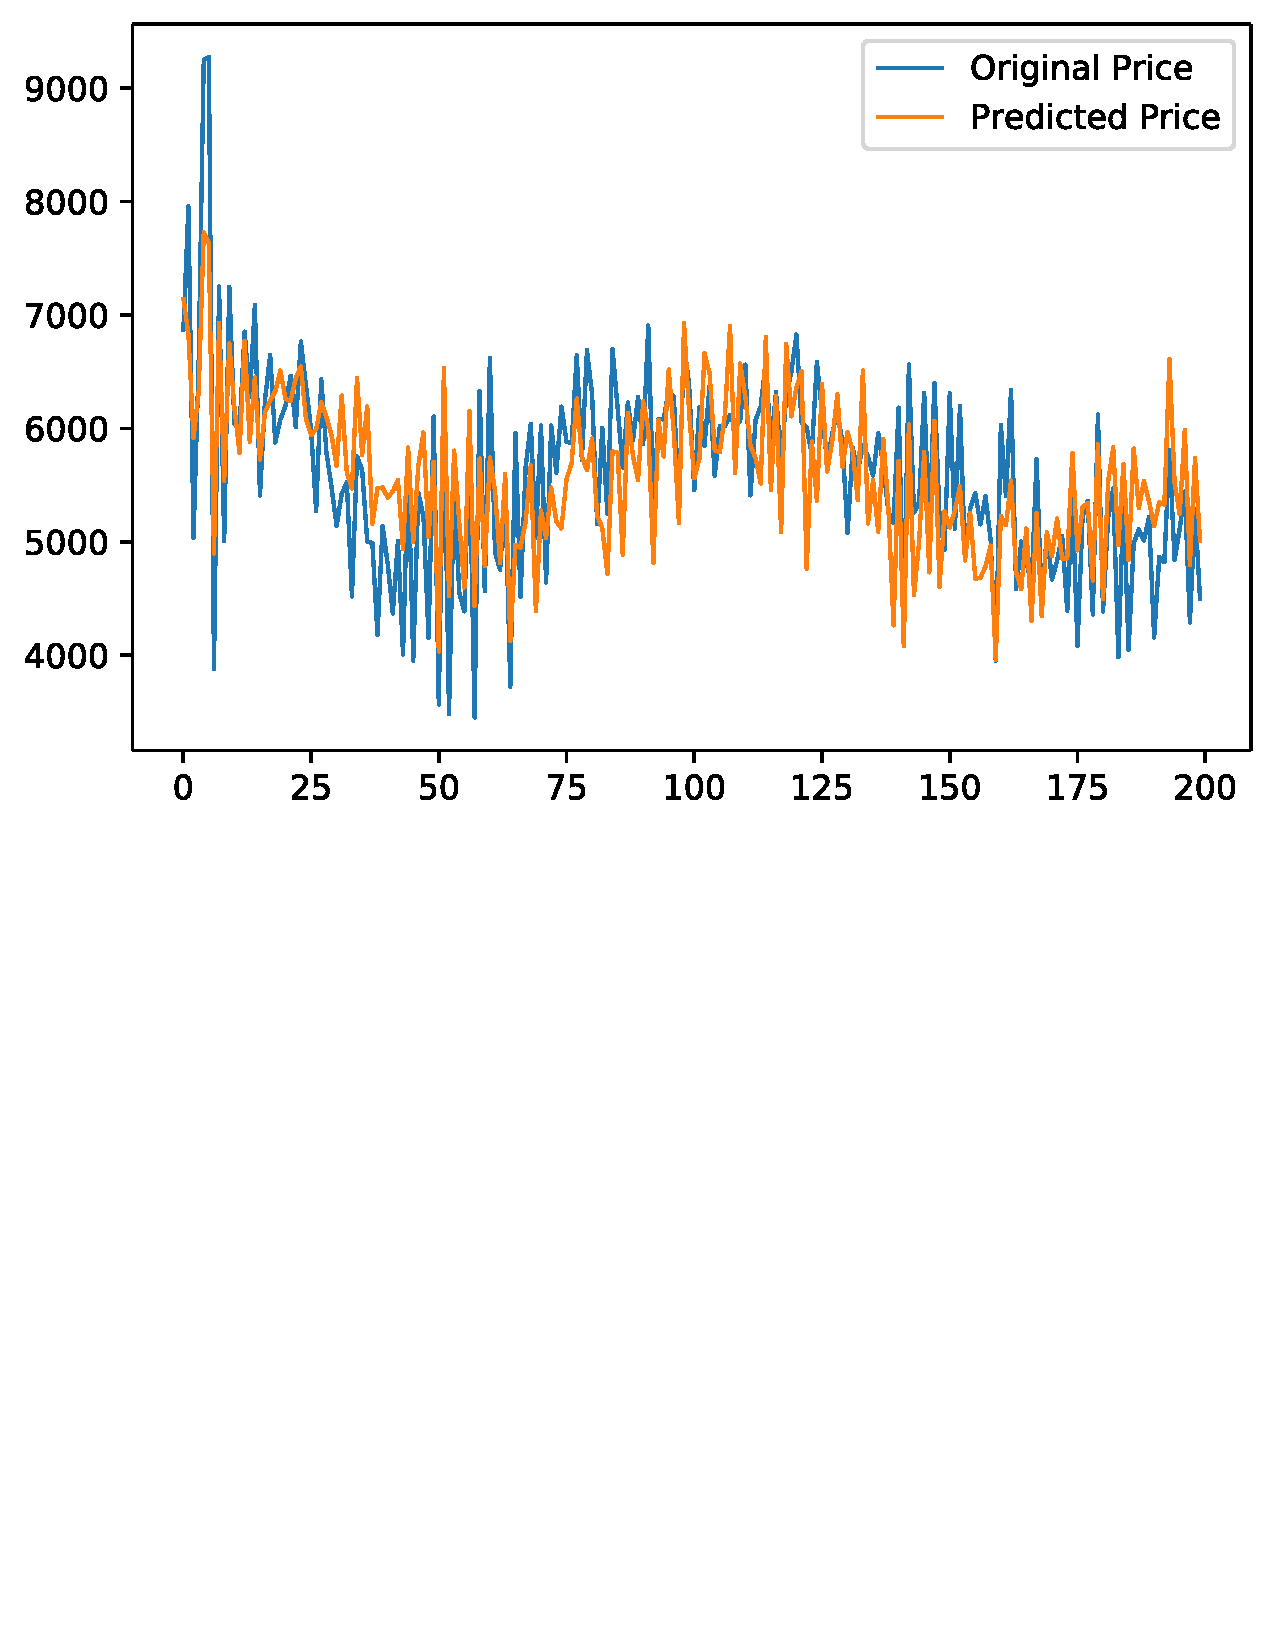
\includegraphics[width=6.5cm]{Fourier_pred.pdf}
	\caption{The predicted price on the training data}
	\label{fig: Fourier Transform}
\end{figure}
\\
\\
And we predict the price on the test data, which looks like:
\\
\\
\begin{figure}[htbp]\centering
	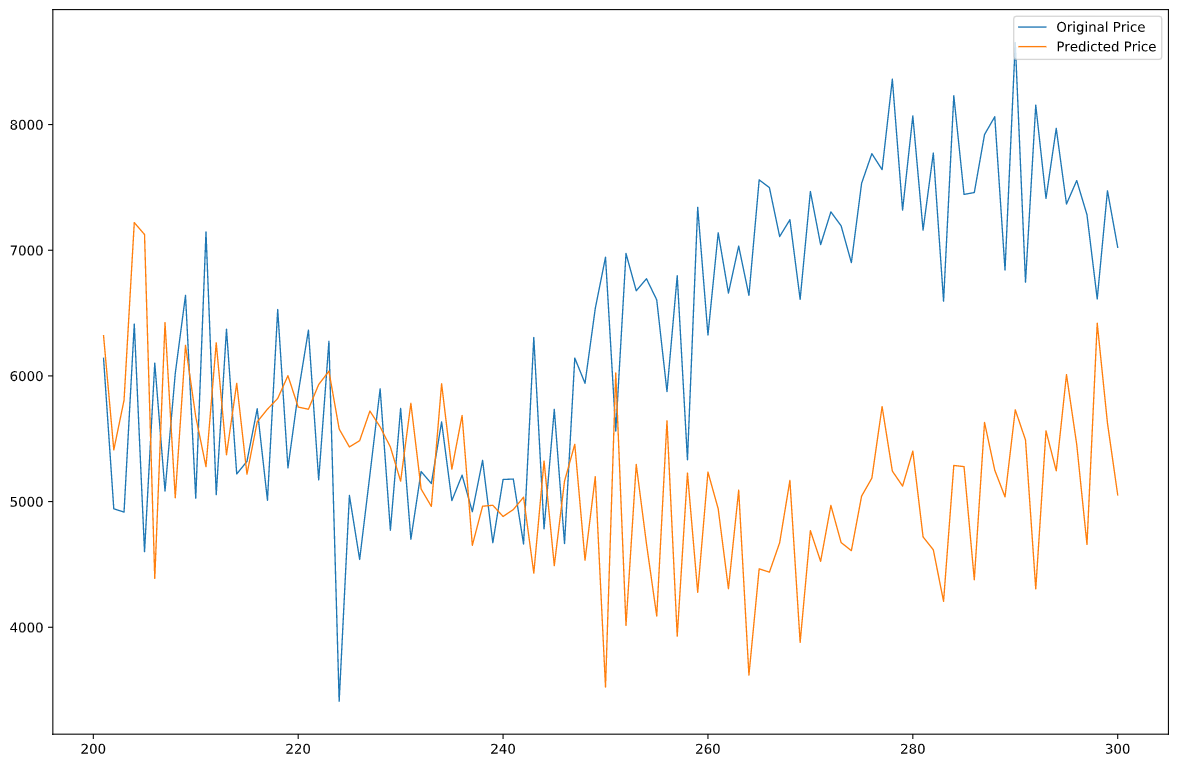
\includegraphics[width=6.5cm]{Fourier_test.png}
	\caption{The predicted price on the test data}
	\label{fig: Fourier Transform}
\end{figure}
\\
\\
The RMSE of this model is 1844.897.
\\
\\
\subsection{Model 3: Taylor Expansion}
The Taylor Expansion requires the model looks like:
\begin{equation}
	X_{t} = \sum_{i=0}^{N}a_{i}t
\end{equation}
which could be done by polynomial regression. The key question in this model is to determine the value of N, which is the degree of the polynomial.
This project used leave-one-out cross validation (LOOCV) to determine the degree of polynomial.
Calculate the average MSE of each degree:
\\
\\
\\
\\
\\
\\
\\
\\
\begin{figure}[htbp]\centering
	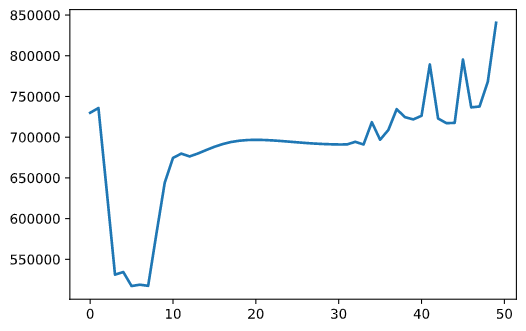
\includegraphics[width=10cm]{CV_AVG.png}
	\caption{The average MSE of each degree}
	\label{fig: Taylor}
\end{figure}
\\
\\
The average MSE of the 6 degree is the smallest. Thus, N = 6. A polynomial regression is performed and the result of prediction is presented as follows:
\\
\\
\begin{figure}[htbp]\centering
	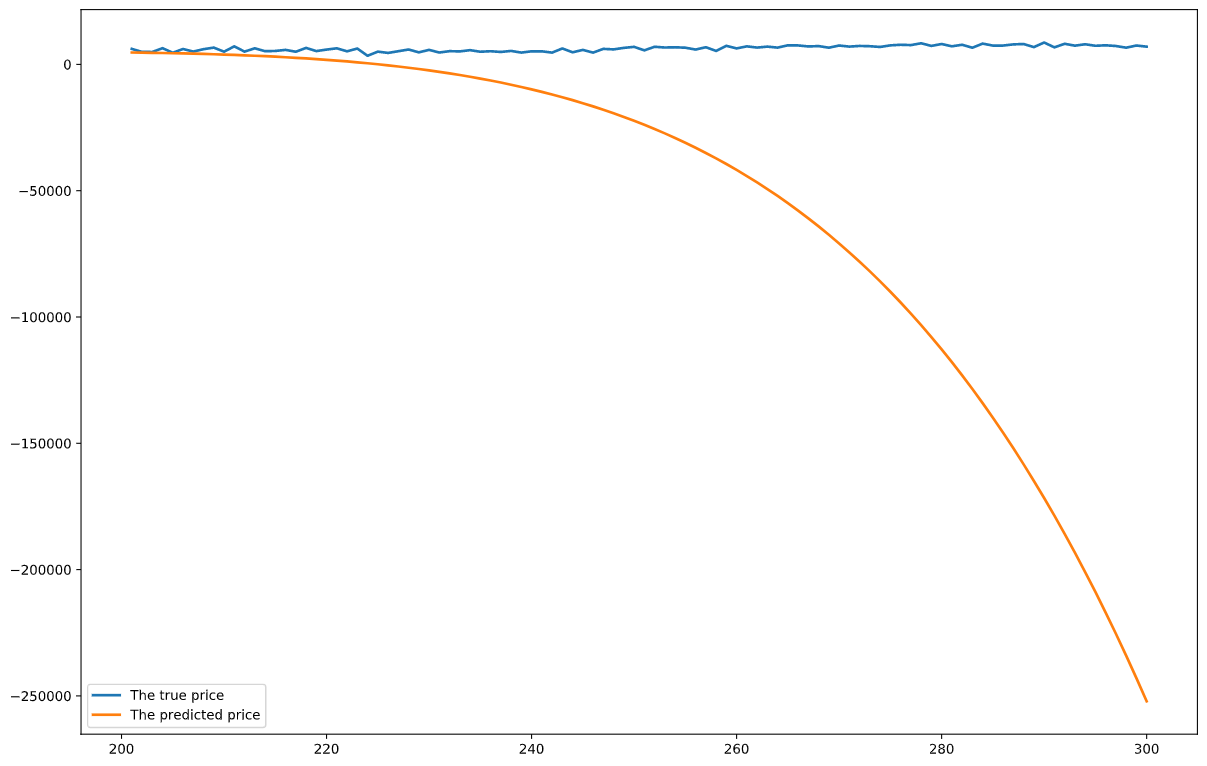
\includegraphics[width=6.5cm]{Taylor_res.png}
	\caption{The result of prediction of Taylor model}
	\label{fig: Taylor}
\end{figure}
\\
\\
The RMSE of the Taylor series is 94479.060.

\subsection{Conclusion}
The autoregression model gives the least RMSE. Thus, this report used Vector Auto Regression Model (VAR) in part 2 of this project. 

\section{Part 2}
The data set of part 2 looks like:
\begin{figure}[htbp]\centering
	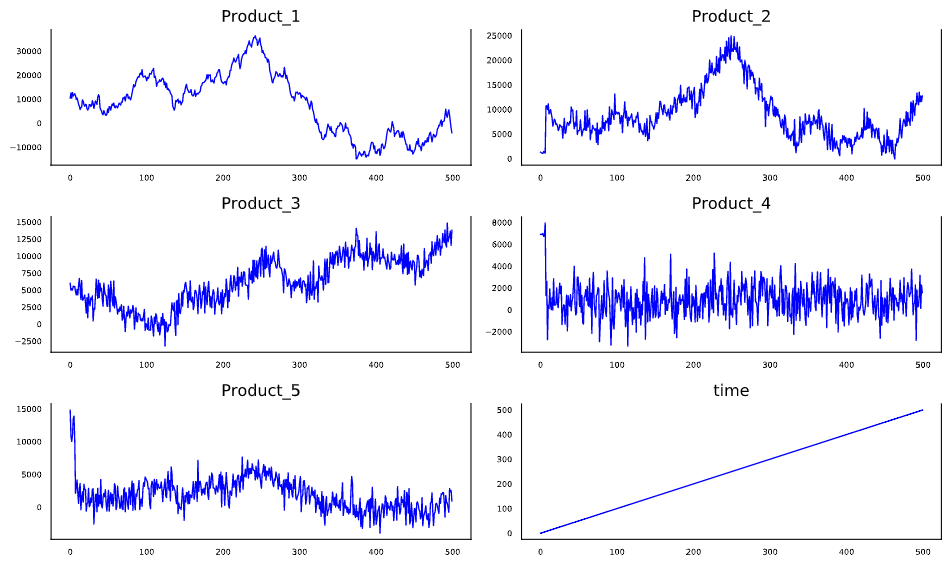
\includegraphics[width=10cm]{Part2.png}
	\caption{The data visualization of part 2}
	\label{fig: VAR}
\end{figure}
Vector autoregression (VAR) is a statistical model used to capture the relationship between multiple quantities as they change over time. A VAR model describes the evolution of a set of k variables, called endogenous variables, over time. Each period of time is numbered, t = 1, ..., T. The k variables are modeled as a linear function of only their past values.
This means we need to solve the least squares estimation of the system:
\begin{equation}
\left[
	\begin{array}[]{c}
		y_{1,t} \\
		y_{2,t} \\
		y_{3,t} \\
		\vdots \\
		y_{k,t} 
	\end{array}
\right]
=
\left[
	\begin{array}[]{c}
		c_{1} \\
		c_{2} \\
		c_{3} \\
		\vdots \\
		c_{k}
	\end{array}
\right]
+
\left[
	\begin{matrix}
		&a_{1,1}^{1}    &a_{1,2}^{1}    &\cdots    &a_{1,k}^{1} \\
		&a_{2,1}^{1}    &a_{2,2}^{1}    &\cdots    &a_{2,k}^{1} \\
		&\vdots         &\vdots         &\vdots    &\vdots\\
		&a_{k,1}^{1}    &a_{k,2}^{1}    &\cdots    &a_{k,k}^{1} \\   
	\end{matrix}
\right]
\left[
	\begin{array}[]{c}
		y_{1, t-1} \\
		y_{2, t-1} \\
		y_{3, t-1} \\
		\vdots \\
		y_{k, t-1}
	\end{array}
\right]
+ \cdots +
\left[
	\begin{matrix}
		&a_{1,1}^{p}    &a_{1,2}^{p}    &\cdots    &a_{1,k}^{p} \\
		&a_{2,1}^{p}    &a_{2,2}^{p}    &\cdots    &a_{2,k}^{p} \\
		&\vdots         &\vdots         &\vdots    &\vdots\\
		&a_{k,1}^{p}    &a_{k,2}^{p}    &\cdots    &a_{k,k}^{p} \\   
	\end{matrix}
\right]
\left[
	\begin{array}[]{c}
		y_{1, t-p} \\
		y_{2, t-p} \\
		y_{3, t-p} \\
		\vdots \\
		y_{k, t-p}
	\end{array}
\right]
\end{equation}
The Vector Auto Regression has a strict assumption on the stationary of the time series.Thus, one test had to be performed, which is Augumented Dickey-Fuller Test. It turned out that price of product 1, product 2, and product 3
are not stationary. We calculate the increment difference of each series and use them to perform an Augumented Dickey-Fuller Test. It turned out that five series are all stationary.
Next, we need to test the correlation between each time series. The test is Granger's Causality Test. The result is presented as follows (The value in the form is the p-value of the test. The null hypothesis is the correlation between time series is 0):
\begin{figure}[htbp]\centering
	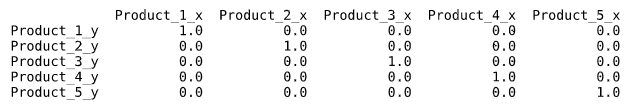
\includegraphics[width=6.5cm]{p-vbalue.png}
	\caption{Granger's Causality Test}
	\label{fig: VAR}
\end{figure}
The key question in this model is the same as the autoregression model, which is to determine the value of p, the number of time lags we use.
This report build the model from lag 1 to lag 80 and found the best lag by AIC. The best lag is 78. 
Finally, we use lag 78 to build and predict the model. The result is presented as follows:
\begin{figure}[htbp]\centering
	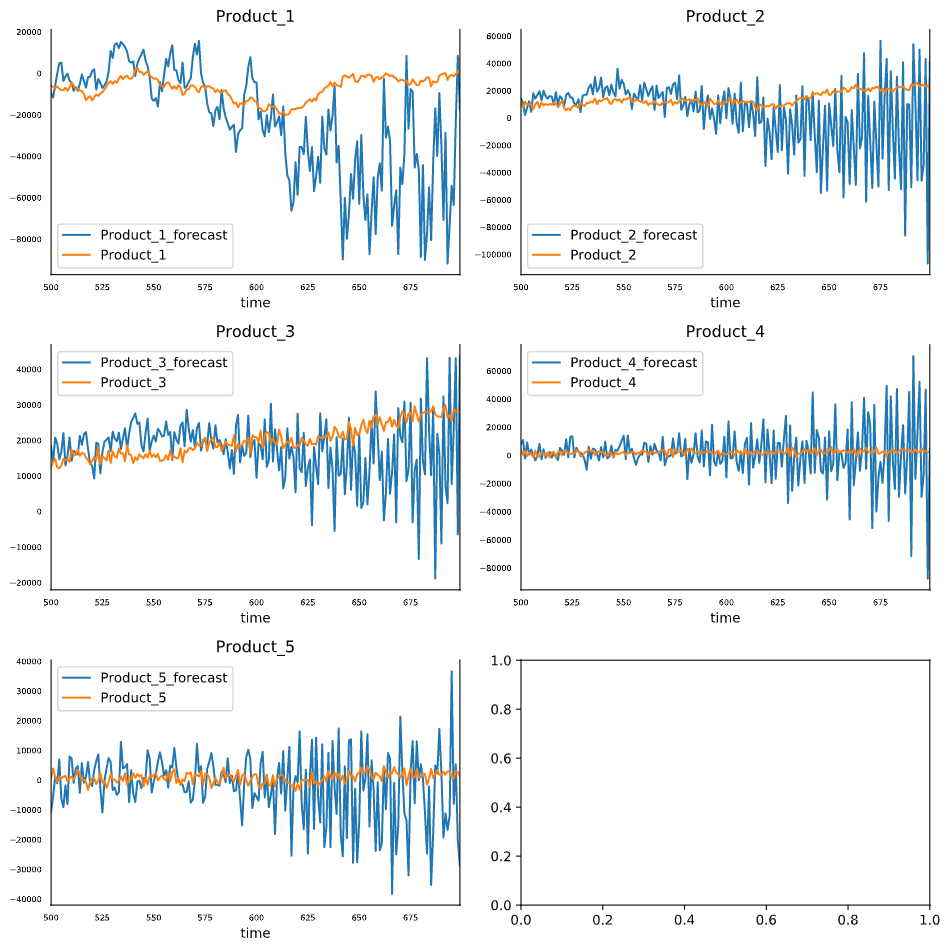
\includegraphics[width=10cm]{Final_res.png}
	\caption{The prediction result of the VAR model}
	\label{fig: VAR}
\end{figure}
The RMSE for each product are:
\begin{itemize}
	\item [1)] product 1: 31976.980883723056
	\item [2)] product 2: 29334.36012630151
	\item [3)] product 3: 10965.563702961275
	\item [4)] product 4: 19445.44243437039
	\item [5)] product 5: 11770.881628593599
\end{itemize}

\textbf{The detailed implementation is shown in the code (written in Python on jupyter notebook)}

\end{document}
